\documentclass{article}
\usepackage{tikz}
\usepackage{tikz-3dplot}
\usetikzlibrary{shapes.geometric,shapes.symbols}
\typeout{STZ PGF VERSION \pgfversion}
\input{tiny-cylinder.sty}
\begin{document}
\makeatletter
\newwrite\domainout\immediate\openout\domainout=domain.txt
\let\originaldivide\pgfmathdivide@
\def\pgfmathdivide@#1#2{\immediate\write\domainout{DIVIDE #1; #2}\originaldivide{#1}{#2}}
\makeatother
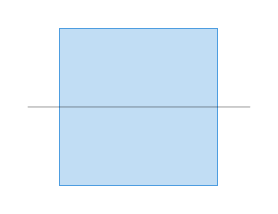
\begin{tikzpicture}[baseline={([yshift=-.5ex]current bounding box.center)}, line cap=round, line join=round]
    %----------------------------------------
    % Styles and colors
    %----------------------------------------
    % TikZ export mode: inline math. Setup is local to this tikzpicture.
    %----------------------------------------
    % Package requirements
    %----------------------------------------
    % Requires \usepackage{tikz-3dplot}
    % Required TikZ libraries for non-circular point shapes:
    % \usetikzlibrary{shapes.geometric,shapes.symbols}
    %----------------------------------------
    % Local colors
    %----------------------------------------
    \definecolor{stzSheetoccludingsheetFill}{HTML}{4D9DE0}
    \definecolor{stzSheetoccludingsheetStroke}{HTML}{4D9DE0}
    \definecolor{stzPointpFill}{HTML}{000000}
    \definecolor{stzPointpStroke}{HTML}{000000}
    \definecolor{stzPointpText}{HTML}{000000}
    %----------------------------------------
    % TikZ layers
    %----------------------------------------
    \pgfdeclarelayer{stratifiedLayer0}
    \pgfsetlayers{stratifiedLayer0,main}
    %----------------------------------------
    % Camera setup
    %----------------------------------------
    \tdplotsetmaincoords{90}{0}
    \begin{scope}[tdplot_main_coords]
        %----------------------------------------
        % Coordinates
        %----------------------------------------
        \coordinate (sheetQuadSheet0Face0p0) at (-1,0,-1);
        \coordinate (sheetQuadSheet0Face0p1) at (1,0,-1);
        \coordinate (sheetQuadSheet0Face0p2) at (1,0,1);
        \coordinate (sheetQuadSheet0Face0p3) at (-1,0,1);
        \coordinate (pointPoint0p0) at (0,-1,0);
        %----------------------------------------
        % Layered drawing commands
        %----------------------------------------
        % Layer 0: stratifiedLayer0
        \begin{pgfonlayer}{stratifiedLayer0}
            %----------------------------------------
            % Codimension 1 strata: sheets
            %----------------------------------------
            % Auto surface face depth sort: sheet "Sheet" [occluding-sheet], face 0, avg depth 0.
            \filldraw[
                fill=stzSheetoccludingsheetFill,
                fill opacity=0.35,
                draw=stzSheetoccludingsheetStroke,
                draw opacity=1
            ]
                (sheetQuadSheet0Face0p0) -- (sheetQuadSheet0Face0p1) -- (sheetQuadSheet0Face0p2) -- (sheetQuadSheet0Face0p3) -- cycle;
            %----------------------------------------
            % Codimension 3 strata: points
            %----------------------------------------
            % Auto point visibility: point "Point" [p] hidden behind sheet [occluding-sheet] face 0 and dimmed.
            \node[
                cylinder,
                fill=stzPointpFill,
                draw=stzPointpStroke,
                text=stzPointpText,
                fill opacity=0.28,
                draw opacity=0.28,
                text opacity=0.28,
                line width=0.4pt,
                solid,
                dash phase=0pt,
                line cap=butt,
                line join=miter,
                inner sep=1.5pt,
                inner xsep=0pt,
                inner ysep=0.000074pt,
                outer xsep=0pt,
                outer ysep=0pt,
                minimum width=0pt,
                minimum height=80pt
            ] at (pointPoint0p0) {};
        \end{pgfonlayer}
        % Codimension 2 strata: curves
        % Labels
    \end{scope}
\end{tikzpicture}
\end{document}
